\begin{appendix}
\chapter{Algoritmo de Grover}\label{sec:Grover}

El algoritmo de Grover es el algoritmo cuántico de búsqueda óptimo en un conjunto desordenado \cite{grover1996fast}, \cite{nielsen2002quantum}. Lo llevamos a cabo con el operador de Grover $\hat{G}$ que es producto de dos operaciones en el espacio de n qubits $\hat{G}=(2\ket{\psi}\bra{\psi}-I)\hat{O}$: (1) el operador $\hat{O}:\ket{x}\xrightarrow{}(-1)^{f(x)}\ket{x}$, donde $f(x)$ es la función oráculo que tiene valor $f(x)=0$ cuando $x$ no es respuesta a la consulta (no es el elemento marcado), y $f(x)=1$ cuando $x$ sí es respuesta. $\hat{O}$ aplica un cambio de fase sobre los elementos marcados del conjunto. (2) el operador $2\ket{\psi}\bra{\psi}-I$ denomiado difusor de Grover.
\begin{equation}
\ket{\psi}=\hat{H}^{\otimes n}\ket{0}=\frac{1}{\sqrt{N}}\sum_{x=0}^{N-1}\ket{x}
\end{equation}
\noindent Es posible un mapeo del espacio de Hilbert de los n qubits sobre los subespacios $\ket{\alpha}$, superposición de los elementos no marcados, y $\ket{\beta}$, superposición de los marcados, es decir $\mathbb{R}^2$, cuyo producto tensorial genera un subespacio en el que $\ket{\psi}$ y $\hat{G}\ket{\psi}$ están contenidos. Ver la gráfica (\ref{gr:Grover}).

\begin{equation}
    \ket{\alpha}=\frac{1}{\sqrt{N-M}}\sum_x\,^{'}\ket{x}\qquad,\qquad    \ket{\beta}=\frac{1}{\sqrt{M}}\sum_x\,^{''}\ket{x}
\end{equation}
$\ket{\psi}$ como combinación de $\ket{\alpha}$ y $\ket{\beta}$ es:
\begin{equation}
\ket{\psi}=\sqrt{\dfrac{N-M}{N}}\ket{\alpha}+\sqrt{\dfrac{M}{N}}\ket{\beta}
\label{ec:GroverInicial}
\end{equation}{}
La aplicación de $\hat{O}$ genera un reflexión alrededor de $\ket{\alpha}$, y $(2\ket{\psi}\bra{\psi}-I)$ una reflexión alrededor de $\ket{\psi}$. Ambas reflexiones generan una rotación como en la gráfica. Llamemos $\cos{\theta/2}=\sqrt{(N-M)/N}$, y $\sin{\theta/2}=\sqrt{M/N}$. La rotación tras una aplicación es $\theta$:

\begin{equation}
    \hat{G}\ket{\psi}=\cos\frac{3\theta}{2}\ket{\alpha}+\sin\frac{3\theta}{2}\ket{\beta}
\end{equation}
En efecto, $\hat{G}$ tiene la representación de una rotación usual en $\mathbb{R}^2$ (como en \ref{MatrizRotaciones}).\\
Si rotamos las veces necesarias hasta estar muy próximos al estado $\ket{\beta}$, una medición tendrá alta probabilidad de resultar en un elemento marcado.
¿Cuántas veces debe operar $\hat{G}$ para que el vector final sea tan próximo a $\ket{\beta}$? Para responder, notemos el ángulo complementario a $\theta/2$: $\arccos\sqrt{M/N}$, entonces la cantidad de rotaciones apropiada es:
\begin{equation}
    R=\text{CI}\big( \dfrac{\arccos\sqrt{M/N}}{\theta}\big)
    \label{ec:RGrover}
\end{equation}

\begin{figure}[ht]
\centering
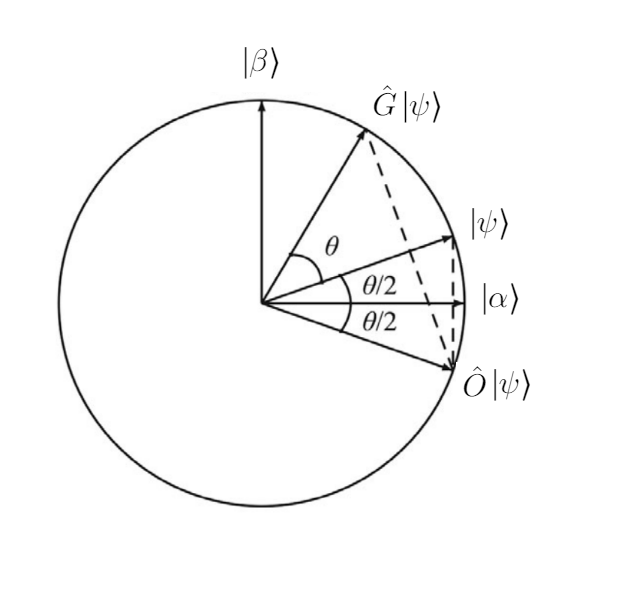
\includegraphics[width=0.6\textwidth]{Anexos/grover.png}
\caption{Grover}
\label{gr:Grover}
\end{figure}
donde $\text{CI}(x)$ es el entero completo de $x$, por ejemplo $\text{CI}(3,72)=3$. Tras aplicar $R$ veces el operador de Grover, el ángulo final sobre $\ket{\beta}$ es $<\pi/4$ y la probabilidad de medir un elemento marcado es significativa, $\pi^2/16>1/2$. El caso particular $M\ll N$ es notorio: $\theta/2\approx \sin(\theta/2)\approx \sqrt{M/N}$, con lo cual $R\approx N/M$, y el error después de la medición es $M/N$. \\
La complejidad del algoritmo es igual al número de rotaciones $R$, ya que cada aplicación tiene el costo de un solo llamado al oráculo. en (\ref{ec:RGrover}) $R$ tiene una cota superior $R=\lceil\pi/2\theta \rceil$, debido al máximo valor posible del numerador. Ahora, una cota inferior de $\theta$ impone otra cota superior sobre $R$.

\begin{equation}
    \frac{\theta}{2}>\sin\frac{\theta}{2}=\sqrt{\frac{M}{N}}
\end{equation}
Así que $R=\mathcal{O}(\frac{\pi}{4}\sqrt{\frac{N}{M}})$

Así que $R=\mathcal{O}(\sqrt{N/M})$ y en el caso de $M=1$, $R=\mathcal{O}(\sqrt{N})$.

\begin{center}
    \begin{tabular}{l}
    \hline \textbf{Algoritmo de Grover}\\\hline
    \textbf{entradas:} \\
    \textbf{salidas:}\\\hline
    \textbf{proceso}\\
    \textbf{1.} [Preparar:] Preparar el estado inicial $\ket{\psi}$ como en (\ref{ec:GroverInicial}).\\
\textbf{2.} Ejecutar lo siguiente $\mathcal{O}(\sqrt{N/M})$ número de veces:\\
(a) [Chequear:] Aplicar $\mathcal{O}$ (reflexión con respecto a $\ket{\alpha}$)\\
(b) [Actualizar:] Aplicar $2\ket{\psi}\bra{\psi}-I$ (reflexión con respecto a $\ket{\psi}$)\\
\textbf{3.} Medir el estado final\\\hline
    \end{tabular}{}
\end{center}{}
%Para el costo en la del algoritmo nos ocupamos del operador $(\ket{\psi}\bra{\psi}-I)$. En cuanto al oráculo sabemos que usarlo hace que el análisis de la eficiencia se base en el número de consultas, y que su implementación es particular al tipo de problema, así que aquí no nos ocupamos de él más allá de contar $R$.\\  Los pasos (1) y (3) tienen cada uno costo de $n$, por su parte, el paso (2) $N=\log n$.
Este algoritmo permite la solución a otros problemas además del de búsqueda exhaustiva de un elemento marcado en una base de datos, por ejemplo, encontrar posibles soluciones al problema del problema del viajante (traveling salesman problem)\footnote{"Dada una lista de ciudades y de distancias entre cada par de ellas, ¿cuál es la ruta más corta posible que visita cada ciudad y regresa a la ciudad de origen?"}, o el problema de distinción de los elementos resueltos por Ambainis.
%Este algoritmo fue probado como óptimo en la búsqueda de un elemento marcado.

\chapter{Solución analítica de la caminata sobre la línea}\label{Anexo:SolucionLinea}
Para encontrar la solución analítica dos análisis son comunes: el primero por integrales de camino (o sumas porque el espacio de posiciones es discreto), que corresponde al análisis por combinatoria [Konno, 2002], y el segundo por transformadas de fourier, lógicamente sugerido por la invarianza espacial. En esta sección presentamos la solución por transformadas de fourier. Este método sirve para analizar otras caminatas sobre gráficas con invarianza espacial de la sección \ref{sec:Graficas}.\\
Escribamos la función de onda para cualquier tiempo de la siguiente forma
\begin{equation}{}
\ket{\Psi(t)}=\sum_{j=0}^1\sum_{x=-\infty}^\infty\psi_{j,k}\ket{j,x},
\end{equation}
que cumple con
\begin{equation}
    \sum_{x=-\infty}^\infty p_x(t)=1,\qquad p_x(t)=|\psi_{0,x}(t)|^2+|\psi_{1,x}(t)|^2.
\end{equation}{}
Operemos $\hat{U}\ket{\Psi(t)}=\hat{S}(\hat{H}\otimes\mathbb{I})\ket{\psi(t)}$,
\begin{equation}{}
    \ket{\Psi(t+1)}=\sum_{x=-\infty}^\infty \frac{1}{\sqrt{2}}(\psi_{0,x}+\psi_{1,x})\ket{0,x-1}+\frac{1}{\sqrt{2}}(\psi_{0,x}-\psi_{1,x})\ket{1,x+1}
\end{equation}{}
Al expandir el lado izquierdo y reorganizar el lado derecho corriendo dos veces el índice $x$, obtenemos la siguiente solución
\begin{align}
    \psi_{0,x}(t+1)=\frac{1}{\sqrt{2}}(\psi_{0,x+1}(t)+\psi_{1,x+1}(t))\\
    \psi_{1,x}(t+1)=\frac{1}{\sqrt{2}}(\psi_{0,x-1}(t)+\psi_{1,x-1}(t))
\end{align}{}
Estas ecuaciones de recurrencia son útiles para simular las amplitudes numéricamente, como aparece en la gráfica (\ref{gr:Hadamard100Simulacion}). Sin embargo es más sencillo desarrollar su solución analítica con transformadas de fourier.
%El ejemplo de la matriz de Pauli $\hat{\sigma_x}$.
Transformamos las amplitudes $\psi_{j,k}$ y los vectores de la base $\ket{k}$,
\begin{equation}
    \widetilde{\psi_j}(k,t)=\sum_{x}e^{-ikx}\psi_{j,k}(t),\qquad ;\qquad
    \widetilde{\ket{k}}=\sum_xe^{ikx}\ket{x},
    \label{T.F.}
\end{equation}{}

%que es infinita pero para hacer $\widetilde{\ket{k}}$ de norma finita se considera el siguiente límite
%\begin{equation}
 %   \widetilde{\ket{k}}=\lim_{L\xrightarrow{}\infty}\frac{1}{\sqrt{2L+1}}\sum_{x=-L}^Le^{ikx}\ket{x}
%\end{equation}{}
%sin embargo, continuamos el trabajo con \ref{T.F.base} y la precaución.
Hemos definido una nueva base ortonormal $\left\{\ket{j,\widetilde{k}}:j\in\{0,1\},-\pi\leq \widetilde{k}\leq\pi\right\}$, sobre la cual podemos expandir cualquier estado:
\begin{equation}{}
\ket{\Psi(t)}=\sum_j\int_{-\pi}^\pi\frac{dk}{2\pi}\widetilde{\psi_j}(k',t)\widetilde{\ket{k}}
\end{equation}
En esta base la operación moneda contiene la información completa de la evolución, lo que significa que hallar su espectro es suficiente para establecer el espectro del operador $\hat{U}$. Primero establezcamos la operación $\hat{S}$ sobre la nueva expansión de la amplitud,
\begin{equation}
    \hat{S}\ket{j,\widetilde{k}}=\sum_xe^{ikx}\ket{j,x+(-1)^{j+1}}=e^{(-1)^{j+1}}\sum_{x'}e^{ikx'}\ket{j,x'}=e^{-(-1)^{j+1}}\ket{j,\widetilde{k}}.
\end{equation}{}
el cambio de variable $x+(-1)^{j+1}\xrightarrow{}x'$ no altera los límites de la suma.\\
$\hat{S}$ es diagonal en la base de Fourier, con autovectores $\ket{j,\widetilde{k}}$ y autovalores $e^{-(-1)^{j+1}}$. Si diagonalizamos el operador $\hat{C}$ también habremos diagonalizado $\hat{U}$. Esto último es sencillo ya que $\hat{C}$ es de dimensión 2. Llamemos $\hat{H}_{j,j'}$ los elementos fila de $\hat{H}$ tal que $\hat{H}_{j,j'}\ket{j}=\ket{j'}$,
\begin{equation}
    \hat{U}\ket{j',\widetilde{k}}=\hat{S}\sum_{j=0}^1\hat{H}_{j,j'}\ket{j,\widetilde{k}}
\end{equation}{}
\begin{equation}
    \bra{j,\widetilde{k}}\hat{U}\ket{j',\widetilde{k'}}=e^{-ik(-1)^{j+1}}\hat{H}_{j,j'}\delta(k-k').
\end{equation}{}
La delta en $k$ pone en claro que los elementos no diagonales de $\hat{U}$ son de $\hat{H}_{j,j'}$. Llamemos $\widetilde{H}_k$ a una nueva matriz con elementos $e^{-ik(-1)^{j+1}}\hat{H}_{j,j'}$, absorbiendo los autovalores de $\hat{S}$.
\begin{equation*}
\hat{H}_k=
\begin{pmatrix}
e^{-ik} & 0\\
0 & e^{ik}\\
\end{pmatrix}
\frac{1}{\sqrt{2}}
\begin{pmatrix}
1 & 1\\
1 & -1\\
\end{pmatrix}
=\frac{1}{\sqrt{2}}
\begin{pmatrix}
e^{-ik} & e^{-ik}\\
e^{ik} & e^{-ik}\\
\end{pmatrix}
\end{equation*}{}
Esta matriz $\hat{\widetilde{H}}_k$ absorbe las fases de la aplicación de $\hat{S}$, así que contiene la información completa de la operación evolución. 
\begin{equation}
\begin{pmatrix}
 &&\dots&&\dots\\
 & e^{-ik} & e^{-ik} & 0   & \dots & \\
& e^{ik}  & e^{-ik} & 0     & \dots\\
& \dots  & 0     & e^{-ik'}& e^{-ik'} &0  &\dots\\
&  \dots   & 0     & e^{ik'} & e^{-ik'} & 0 &  \dots\\
&      &     & \dots & 0 & e^{-ik''} & \dots \\
&  &  & & \vdots \\
\end{pmatrix}
\end{equation}{}
Si $\alpha_k,\beta_k$, y $\ket{\alpha_k},\ket{\beta_k}$ son los autovalores y autovectores de $\hat{\widetilde{H}}_k$, lo son también de $\hat{U}$.
\begin{equation}
    \hat{U}\ket{j,\widetilde{k}}=\hat{\widetilde{H}}_k\ket{j,\widetilde{k}}=(\hat{\widetilde{H}}_k\ket{\alpha}\ket{\widetilde{k}})=\alpha_k\ket{\alpha_k}\ket{\widetilde{k}}
\end{equation}{}
El polinomio característico de $\hat{\widetilde{H}}_k$ es $\lambda^2+\sqrt{2}i\lambda\sin{k}-1=0$ que dan como autovalores $\alpha_k=e^{-i\omega_k},\beta_k=e^{i(\pi+\omega_k)}$, donde $\omega_k\in[-\pi/2,\pi/2]$, y $\sin\omega_k=\frac{1}{\sqrt{2}}\sin k$. Los autovectores normalizados son:
\begin{align}
    \ket{\alpha_k}=\frac{1}{\sqrt{c^-}}
    \begin{pmatrix}
    e^{-ik}\\
    \sqrt{2}e^{-i\omega_k}-e^{-ik}
    \end{pmatrix}{}
    \label{AutoVector1}
    \\
    \ket{\beta_k}=\frac{1}{\sqrt{c^+}}
    \begin{pmatrix}
    e^{-ik}\\
    -\sqrt{2}e^{i\omega_k}-e^{-ik}
    \end{pmatrix}{}
    \label{AutoVector2}
\end{align}{}
con $c^{\pm}=2(1+\cos ^2k)\pm2\cos k\sqrt{1+\cos ^2k}$. Finalmente, la descomposición espectral de $\hat{U}$
\begin{equation}
    \hat{U}^t=\int_{-\pi}^\pi\frac{dk}{2\pi}\left(e^{-i\omega_kt}\ket{\alpha_k,\widetilde{k}}\bra{\alpha_k,\widetilde{k}}+e^{i(\pi+\omega_k)t}\ket{\beta_k,\widetilde{k}}\bra{\beta_k,\widetilde{k}}\right)
\end{equation}{}

Supongamos que el estado inicial es $\ket{\psi_{in}}=\ket{0,x=0}$, que es la misma condición inicial que usamos para la tabla \ref{TablaCuantica}. Al aplicar $\hat{U}^t$ debemos tener en cuenta $\braket{\alpha_k,\widetilde{k}}{0,0}=e^{ik}/\sqrt{c^-}$ y $\braket{\beta_k,\widetilde{k}}{0,0}=e^{ik}/\sqrt{c^+}$. Entonces,

\begin{equation}
\ket{\psi(t)}= \int_{-\pi}^\pi \frac{dk}{2\pi} \big(\frac{e^{-i(\omega_kt-k)}}{\sqrt{c^-}}\ket{\alpha_k}+\frac{e^{i(\pi+\omega_k)t+ik}}{\sqrt{c^+}}\ket{\beta_k}\big)
\end{equation}{}
A continuación escribimos el estado en amplitudes $\psi_L$ y $\psi_R$, es decir en la base computacional usando (\ref{AutoVector1})  y (\ref{AutoVector2}). Podemos llegar a la solución estándar dada por ejemplo en \cite{portugal2013quantum} ó \cite{nayak2000quantum}, con algo más de álgebra, teniendo en cuenta dos identidades matemáticas:
\begin{equation}
    \frac{1}{c^\pm}=\frac{1}{2}\bigg(1\mp\frac{\cos k}{\sqrt{1+\cos ^2k}} \bigg)    \qquad;\qquad \sqrt{2}e^{i\omega_k}\pm e^{-ik}=\frac{c^\pm}{2\sqrt{1+\cos^2{k}}}
\end{equation}{}
\begin{align}
    \widetilde{\Psi}_L(k,t)&=\frac{1}{2}(1+\dfrac{\cos{k}}{\sqrt{1+\cos^2{k}}})e^{-i\omega_kt}+\dfrac{(-1)^t}{2}(1-\dfrac{\cos{k}}{\sqrt{1+\cos^2{k}}})e^{-i\omega_kt}\\
    \widetilde{\Psi}_R(k,t)&=\frac{ie^{ik}}{2\sqrt{1+\cos^2{k}}}(e^{-i\omega_kt}-(-1)^te^{i\omega_kt})
\end{align}{}
de las cuales se puede obtener las amplitudes en el espacio real con la transformadad inversa.
\begin{align}
    \Psi_L(x,t)&=\dfrac{1+(-1)^{x+t}}{2}\int_{-\pi}^\pi\frac{dk}{2\pi}(1+\frac{\cos k}{\sqrt{1+\cos^2 k}})e^{-i(\omega_kt+kx)}
    \label{ec:AmplitudIzquierda}\\
    \Psi_R(x,t)&=\dfrac{1+(-1)^{x+t}}{2}\int_{-\pi}^\pi\frac{dk}{2\pi}\frac{e^{ik}}{\sqrt{1+\cos^2 k}}e^{-i(\omega_kt+kx)}
    \label{ec:AmplitudDerecha}
\end{align}{}
La probabilidad es $P(x,t)=|\Psi_L(x,t)|^2+|\Psi_R(x,t)|^2$. En la siguiente sección presentamos una aproximación al término de mayor orden de esta probalidad a través del método de fase estacionaria.

\subsubsection{Sobre la solución}
En \cite{nayak2000quantum} se estudia el comportamiento las soluciones (\ref{ec:AmplitudIzquierda}) y (\ref{ec:AmplitudDerecha}), basado en la variable $\alpha)n/t$. La gráfica se divide en tres partes:
\begin{itemize}
    \item para $|\alpha|>\frac{1}{\sqrt{2}}+\mathcal{O}(t^{-2/3})$ decae más rápido que cualquier polinomio inverso en $t$ 
    \item va como $t^{-1/3}$ en un intervalo $\mathcal{O}(t^{-2/3})$ alrededor de $\alpha=\pm 1/\sqrt{2}$
    \item $t^{-1/2}$ en el intervalo restante.
\end{itemize}
Por otra parte, en \cite{nayak2000quantum} obtienen las siguientes expresiones asintóticas a través del método de fase estacionaria:
\begin{equation}
\left.
\begin{array}{cc}
    \Psi_L(\alpha t) \\
    \Psi_R(\alpha t) 
\end{array}{}    
\right\}
= \frac{1+(-1)^{(\alpha+1)t}}{\sqrt{2\pi t|\omega_{k_\alpha}''|}}\times
\left\{
\begin{array}{ll}
     (1-\alpha) \cos{(\phi(\alpha)t+\pi/4)}\\
    \alpha\cos{(\phi(\alpha)t+\pi/4)}-\sqrt{1-2\alpha^2}\sin{(\phi(\alpha)t+\pi/4)}
\end{array}{}
\right.
\end{equation}
\begin{align}
    P(\alpha,t)&=|\Psi_L(\alpha t,t)|^2+|\Psi_R(\alpha t,t)|^2\\
    &\sim\frac{1+(-1)^{(\alpha+1)t}}{\pi+|\omega_{k_\alpha}''|}\times[(1-\alpha)^2\cos^2{(\phi(\alpha)t+\pi/4)}+(1-\alpha)^2\cos^2{(\phi(\alpha)t+k_\alpha+\pi/4)} ]
\end{align}{}
donde $\phi(\alpha)=-\omega_{k_\alpha}-\alpha k_\alpha$, y $k_\alpha$ es la raíz de $\omega_k'+\alpha$ en $[0,\pi]$.
La varianza se obtiene a través de la siguiente expresión para $P$:
\begin{equation}
P(\alpha,t)=P_{\mbox{slow}}(\alpha,t)+P_{\mbox{fast}}(\alpha,t)
\end{equation}{}
\begin{equation}
P_{\mbox{slow}}(\alpha,t)=\frac{1-\alpha}{\pi+|\omega_{k_\alpha}''|}
\end{equation}{}
Se demuestra que cualquier contribución al momento por parte de $P_{\mbox{fast}}$ es de menor orden que $t$ en relación a la contribución de $P_{\mbox{slow}}$
\begin{table}[ht]
    \centering
    \begin{tabular}{|c|c|c|}
    \hline    & $p(\alpha)$ & simulación \\\hline\hline
    $<\alpha>$& $-1+1/\sqrt{2}$=$-0.293$ & $-0.293$ \\\hline   
    $<|\alpha|>$ & $1/2$ & $0.500$ \\\hline
    $<\alpha^2>$ & $1-1/\sqrt{2} =0.293$ & $0.293$\\\hline
    \end{tabular}
    \caption{$p(\alpha)$}
    \label{Momentos}
\end{table}{}
$\sigma^2\sim N^2$, then the expectation position from the distance goes linearly with time, $\sigma\sim N$, and this is quadratically faster than the classical counterpart.
In particular, they have calculated the the asymptotic
behavior of the probability distributions for the walk on the infinite line, and shown that the probability distribution a t time t is within a constant in total variation distance from the uniform distribution over an interval which is of length linear in t.


\end{appendix}